136. \begin{figure}[ht!]
\center{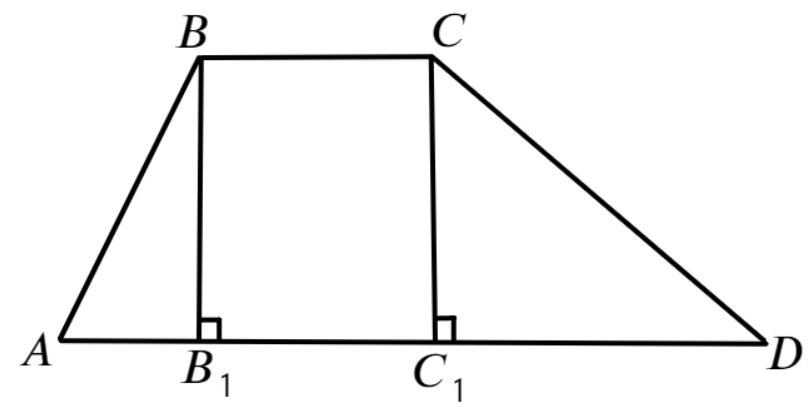
\includegraphics[scale=0.35]{g9-136.png}}
\end{figure}\\
Опустим высоты $BB_1$ и $CC_1.$ Пусть $AB_1=x,$ тогда $C_1D=44-16-x=28-x$ и по теореме Пифагора $BB_1^2=289-x^2=CC_1^2=625-(28-x)^2,$ откуда
$289-x^2=625-784+56x-x^2,\ x=8.$ Тогда $BB_1=\sqrt{289-64}=15$ и $S_{ABCD}=15\cdot\cfrac{16+44}{2}=450.$\\
